\section{LOS Coverage Map}\label{sec:los_map}
A point of interest of the project is to know if there is Line-Of-Sight (LOS) between the ground station (GS) and the UAV. This has been done on a topographic map which takes into account:

\begin{itemize}
	\item Terrain elevation
	\item Curvature of the Earth
	\item Height of receiver and transmitter
\end{itemize}

\subsection{Mathematical Background}
Should this be here ??? or relate with something from the Frames Chapter ???

\subsection{Initial Step}
In this sense, a MATLAB script has been addressed which at first imports a Web Map Service (WMS) to load the topographic map. The map captures the terrain in Denmark and some of its surroundings as seen in Figure \ref{fig:dk_map}.

\begin{figure}[h]
	\centering
	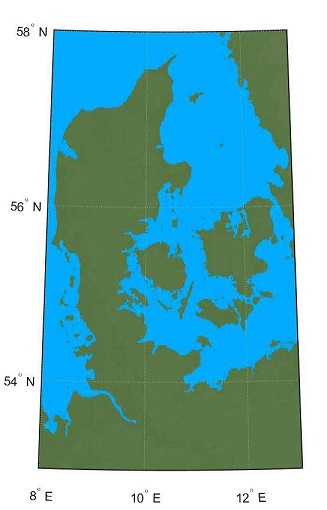
\includegraphics[scale=2]{figures/denmark.jpg}
	\caption{Topographic map of Denmark}
   	\label{fig:dk_map}
\end{figure}

\subsection{LOS Distance}
Given the map and the topographic data in Figure \ref{fig:dk_map}, now it is possible to input the desired points for the GS and the UAV. As mentioned above, there are some parameters taken into account for plotting the LOS distance between the two points of interest. This distance can be seen in Figure \ref{fig:los_2p}, where the LOS is lost after 45 kilometers from the GS.

\begin{figure}[h]
	\centering
	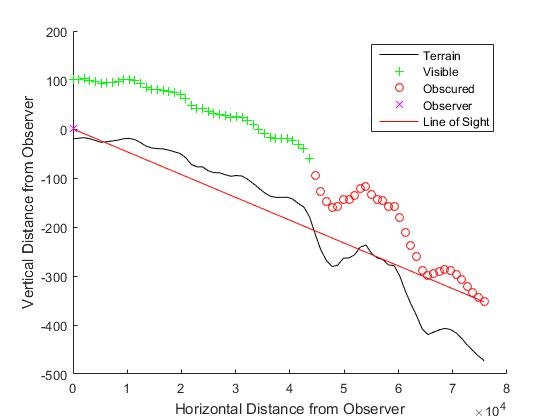
\includegraphics[scale=0.75]{figures/los_2p.jpg}
	\caption{LOS between GS and UAV \\ X axis - LOS distance [m] \\ Y axis - Altitude [m]}
   	\label{fig:los_2p}
\end{figure}

\subsection{Coverage Map}
Moving further, for the same map (Figure \ref{fig:dk_map}) a location for the GS can be chosen, such that it will result into a LOS area (white zone) as seen in Figure \ref{fig:los_area}. This area is also referred as the LOS coverage map.

\begin{figure}[h]
	\centering
	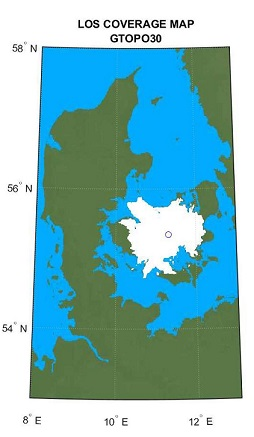
\includegraphics[scale=2.5]{figures/coverage_map.jpg}
	\caption{LOS Coverage Map from the GS}
   	\label{fig:los_area}
\end{figure}

It can be observed from Figure \ref{fig:los_area} that in some areas of the map there is no visibility, due to higher terrain elevation. This can be overcome by increasing the GS and/or UAV altitude, such that we achieve LOS.  


!!! !!! !!! NEED EXAMPLE OF COAST !!! !!! !!!

\subsection{Working Principle}
Taking into account that a MATLAB script has been achieved, a thourough working principle has to be addressed in the following steps:
\begin{itemize}
	\item Aquire topography map 
	\item Input GS and UAV altitudes
	\item Choose locations for GS and UAV on (click) the map in order to plot LOS distance
	\item Choose (click) location of the GS in order to plot LOS coverage map
\end{itemize}